\section{Design}

%$$$$$$$$$$$$$$$$$$$$$$$$$$$$$$$$$$$$$$$$$$$$$$$$$$$$$$$$$$$$$$$$$$$$$$$$$$$$$$$$
%Paragraph 1: LDU의 특징을 간단한 설명과 이번장에 대한 설명(LDU의 특징을 요약하여 설명)
%$$$$$$$$$$$$$$$$$$$$$$$$$$$$$$$$$$$$$$$$$$$$$$$$$$$$$$$$$$$$$$$$$$$$$$$$$$$$$$$$

The LDU is a log-based concurrent updates method to remove scalability
bottlenecks for the update-heavy data structure.
The previous research using the synchronized timestamp counters method may incur
timestamp merging and ordering process.
Therefore, when core counts increases, the timestamp merging and ordering
process may require sequential processing, which can limit scalalbility and
performance.
The LDU can solve these sequential processing.
LDU instantly removes operation logs at update time that require timestamp
counter and reuses the garbage log instead of creating new log
thereby eliminating the synchronized timestamp counter and cache communication
bottleneck.
This section explains these algorithmic design aspects of LDU.

\subsection{Approach}

\begin{figure*}[tb]
  \begin{center}
     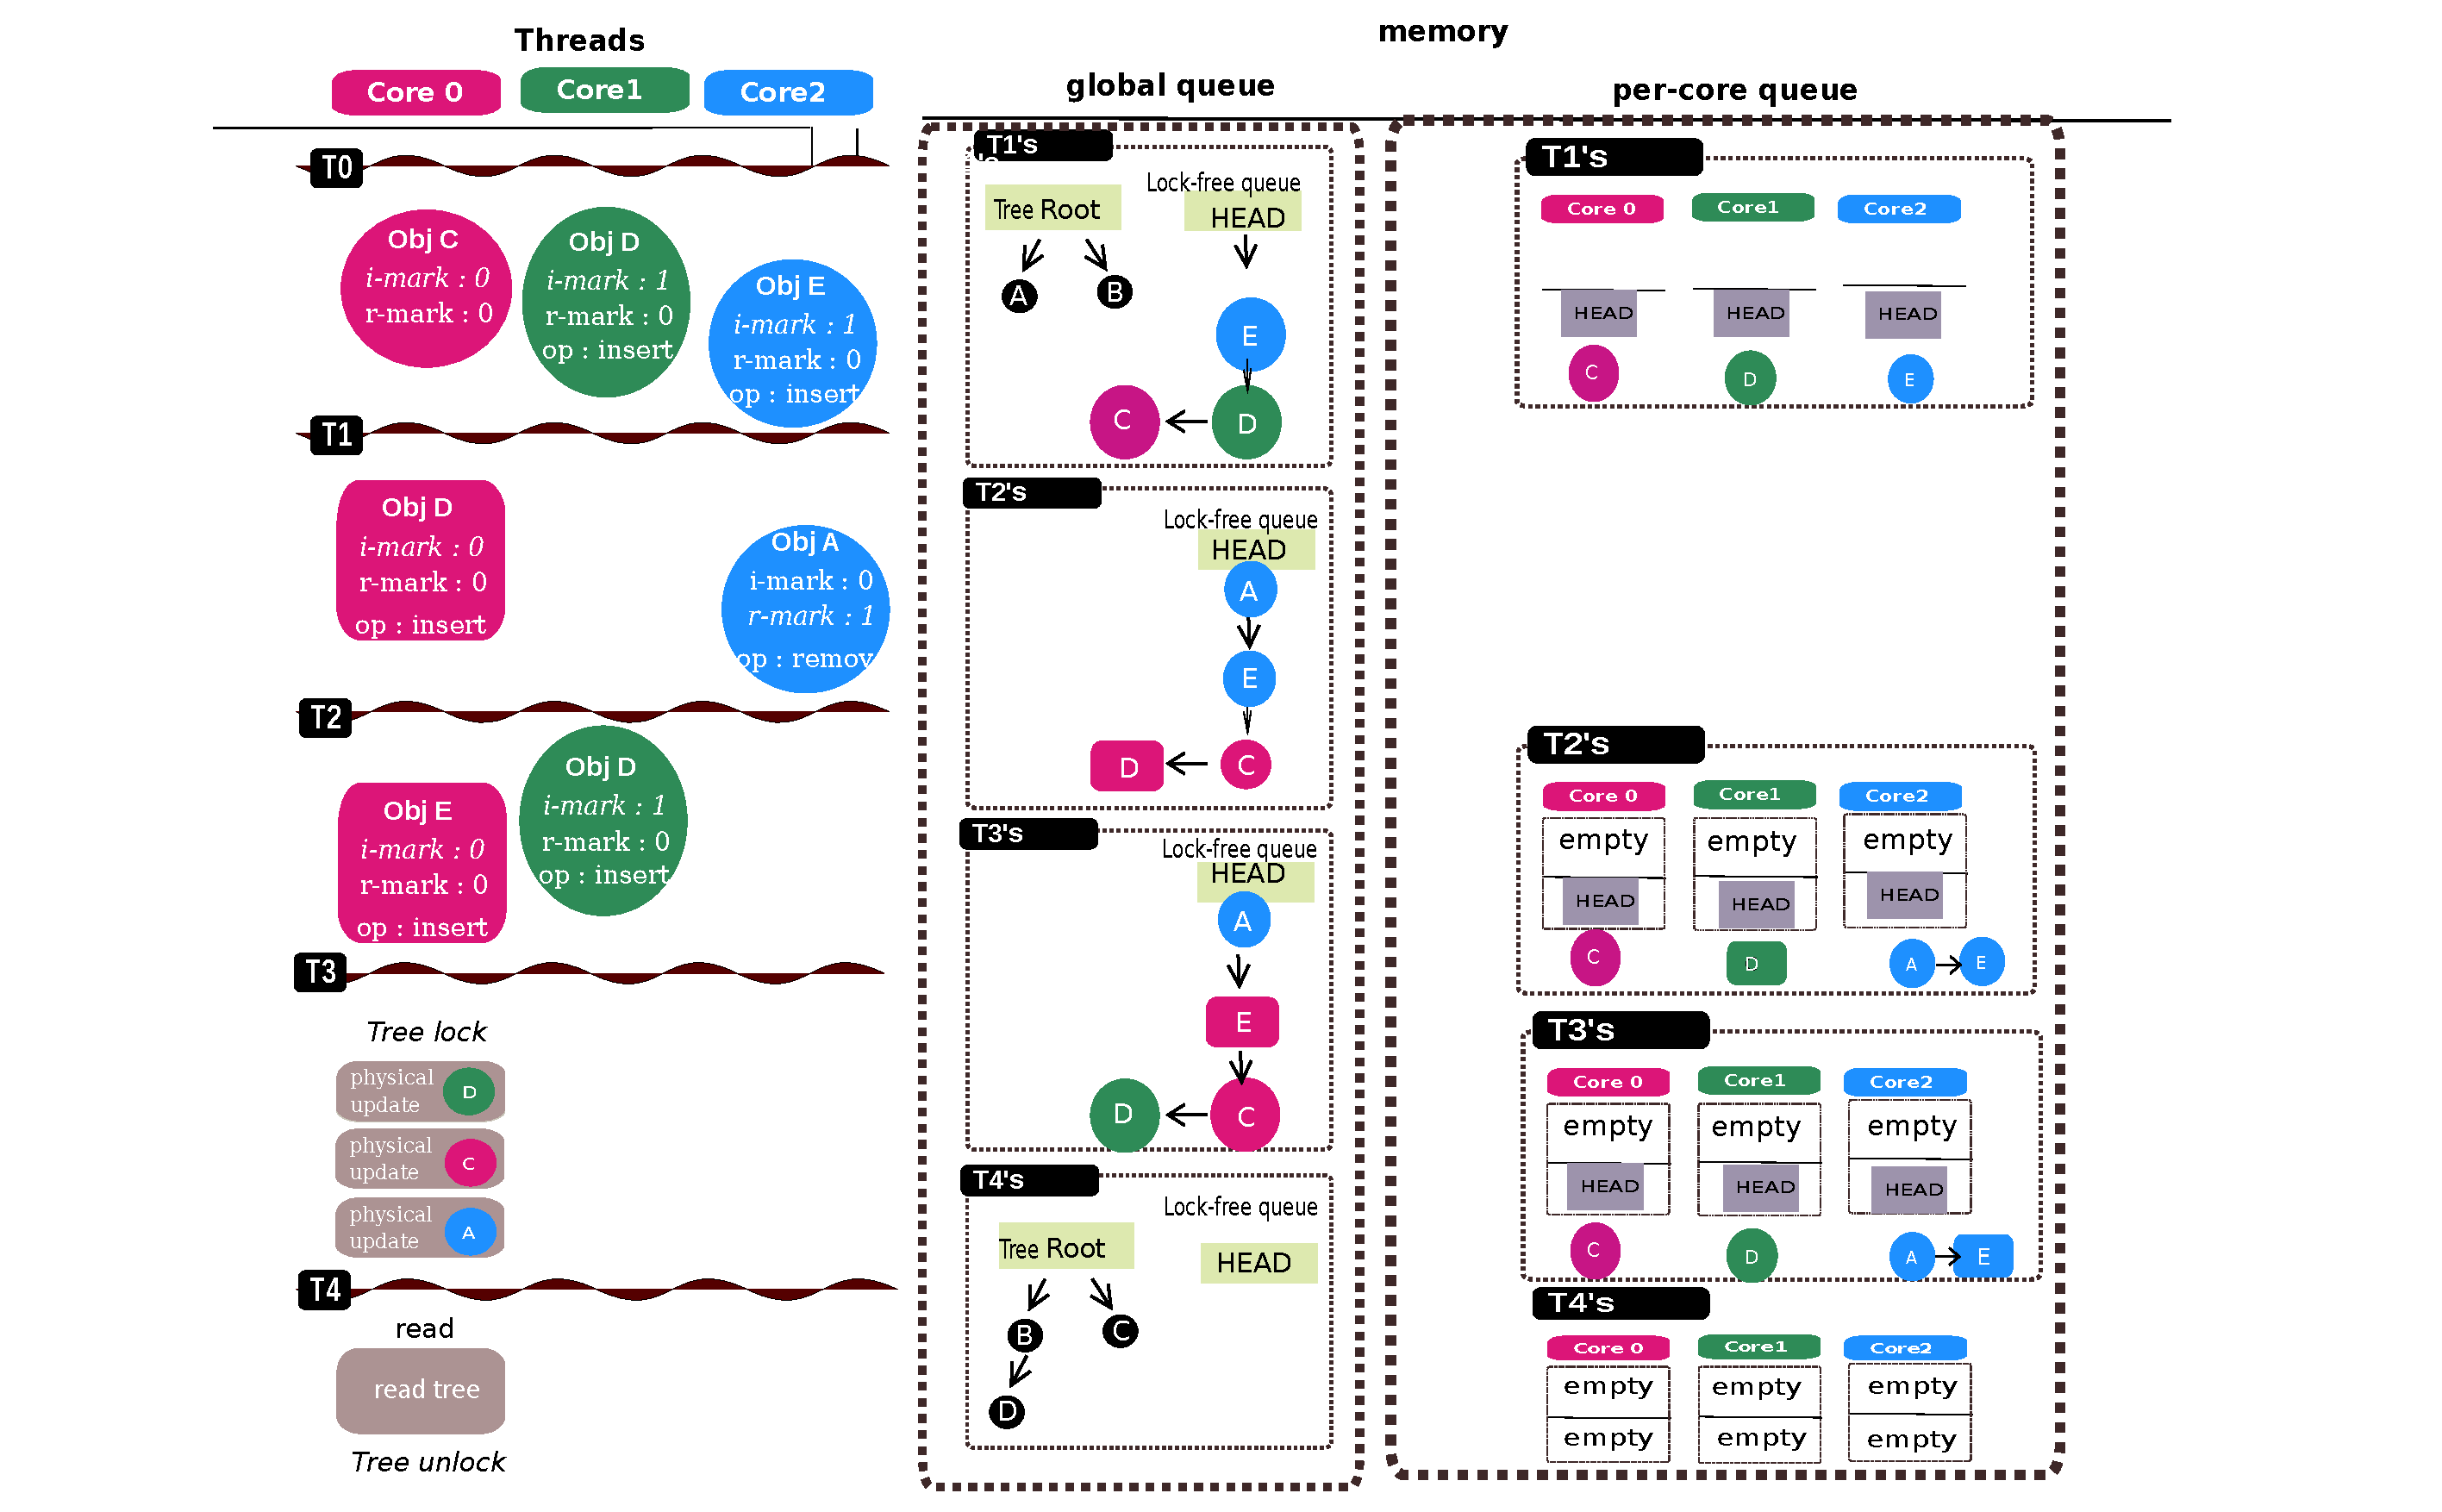
\includegraphics[width=1.0\textwidth,height=0.4\textheight]{fig/basic_gldu}
  \end{center}
  \caption{\deferu example showing seven update operations(insert C, insert D ,
  insert E, remove D, insert A, insert D, and remove E) and one read
  operation. The execution flows from top to bottom.
  Memory represents original data structure and logging queue at T1, T2, T3 and T4, respectively. The early
  the tree data structure contains two object, A and B , and queue is empty.
  The seven update operations concurrently execute without locks and a single
  reader executes with lock.}
  \label{fig:basic}
\end{figure*}

%$$$$$$$$$$$$$$$$$$$$$$$$$$$$$$$$$$$$$$$$$$$$$$$$$$$$$$$$$$$$$$$$$$$$$$$$$$$$$$$$
%Paragraph 2: timestamp가 필요한 이유 : time-sensitive update operation log.
%$$$$$$$$$$$$$$$$$$$$$$$$$$$$$$$$$$$$$$$$$$$$$$$$$$$$$$$$$$$$$$$$$$$$$$$$$$$$$$$$
The fundamental reason for requiring synchronized timestamp counters is some
operations need to be ordered.
For example, a process logs an insert operation to the per-core memory, then
migrates to another core, and logs a remove operation, which must eventually
execute after the insert operation[].
Thus, the synchronized timestamp counters are needed.
To specifically explain this time-sensitive log, we use the symbol label used by
this paper~\cite{Clements15SCR}.
We describe insert as plus-circles $\oplus$, remove as minus-circles
$\ominus$ and object as color-circles \inv{2}{B}(object B). 
Color and vertical offset differentiate cpus.
For example
\begin{center}
$\oplus$\inv{1}{A}, $\oplus$\inv{2}{B}, $\oplus$\inv{3}{C},$\ominus$\inv{2}{A},
$\ominus$\inv{3}{C}, $\oplus$\inv{3}{A}, $\oplus$\inv{3}{C},$\ominus$\inv{1}{C}
\end{center}
consists of five insert operations, three remove operation, three cpus, and
three objects.
This example show that $\oplus$\inv{1}{A} and $\ominus$\inv{2}{A},
time-sensitive log, must be executed in chronological order.
LDU can eliminates this time-sensitive log at update time, so LDU can removes
the synchronized timestamp counters.
One more important fact that these time-sensitive operation logs may be removed
by optimization phase.
For example, insert-remove operations or remove-insert operations such as 
$\ominus$\inv{2}{B}, $\oplus$\inv{3}{C} are the cancelable operations before
the read, so eventually remaining operation logs such as
\begin{center}
 $\oplus$\inv{2}{B}, $\oplus$\inv{3}{A}
\end{center}
are non-time-sensitive logs.
When updates operation occurs, LDU removes these time-sensitive log using
the update-side removing technique.

%$$$$$$$$$$$$$$$$$$$$$$$$$$$$$$$$$$$$$$$$$$$$$$$$$$$$$$$$$$$$$$$$$$$$$$$$$$$$$$$$
%Paragraph 3:  time-sensitive update operation 삭제 방법: Update-side Abosrbing 
%$$$$$$$$$$$$$$$$$$$$$$$$$$$$$$$$$$$$$$$$$$$$$$$$$$$$$$$$$$$$$$$$$$$$$$$$$$$$$$$$

To remove the time-senstivive log, LDU uses the update-side removing scheme.
If insert-remove operations occur in terms of the same object, the scheme will
remove the insert-remove operations at update time.
The OpLog also optimizes by removing the existing operation rather than
adding the new one, but OpLog can not remove log when a thread 
migrates other core, so it needs additional sequntial processing for
the optimization.
LDU, however, have no problem with migrating other core during logging because
it uses the shared atomic swap operation in the indivisual object.


%$$$$$$$$$$$$$$$$$$$$$$$$$$$$$$$$$$$$$$$$$$$$$$$$$$$$$$$$$$$$$$$$$$$$$$$$$$$$$$$$
%Paragraph 5: 리눅스의 Update-side removing 수행 방법
%$$$$$$$$$$$$$$$$$$$$$$$$$$$$$$$$$$$$$$$$$$$$$$$$$$$$$$$$$$$$$$$$$$$$$$$$$$$$$$$$
The update-side removing logs scheme performs atomic swap operation in an
individual object for shared memory systems.
This atomic swap operation alows update operations to atomically remove with the
previous cancelable log.
To achieve update-side removing log, first adds the mark field in the object
structure then use it as a status flag. 
For example, consider the insert-remove operation sequence at the same object.
The first insert operation marks the feild of mark and then the opepration logs
in the queue.
Then, the remove operation occur, LDU does not logs;it just proceed with
changing the mark feild.
When the reader applies logs, LDU applies the logs to the original data
structure in case of the true value of marking feild.
The benefit of this update-side removing scheme is twofold:not only it can
eliminate the time-sensitive operation but also it can cancel the previous
operation log in the queue.

%$$$$$$$$$$$$$$$$$$$$$$$$$$$$$$$$$$$$$$$$$$$$$$$$$$$$$$$$$$$$$$$$$$$$$$$$$$$$$$$$
%Paragraph 7: 또 최적화 방법 reusing garbage object : 
%$$$$$$$$$$$$$$$$$$$$$$$$$$$$$$$$$$$$$$$$$$$$$$$$$$$$$$$$$$$$$$$$$$$$$$$$$$$$$$$$

The second technique, called reusing garbage logs, reuses the garbage log
instead of creating a new log.
The garbage log is already canceled by using the update-side removing scheme,
but it has remained queue.
For example, consider the insert-remove-insert operation.
After the sencond remove operation, the log has remained in the queue, but it is 
already canceled by using update-side removing, hence insert mark filed
has remained zero in the queue.
In this case, the third insert operation reuses the log in the queue instead of 
creating a new log using atomic swap, so it can reduece not only the memory
overhead but also the queueing overhead.

%$$$$$$$$$$$$$$$$$$$$$$$$$$$$$$$$$$$$$$$$$$$$$$$$$$$$$$$$$$$$$$$$$$$$$$$$$$$$$$$$
%Paragraph 8: LDU의 로그는 두 종류의 queue에 저장할 수 있도록 지원
%$$$$$$$$$$$$$$$$$$$$$$$$$$$$$$$$$$$$$$$$$$$$$$$$$$$$$$$$$$$$$$$$$$$$$$$$$$$$$$$$
We designs the log's queue using both the per-core and the global queue becasue
it can further support various data structures.
The per-core queue of the LDU can remove the CAS operations that access global
head pointer. 
However, the per-core queue does not properly apply to all data structures since
it has some drawbacks.
The per-core queue has a memory overhead, and developers may need
an additional management code for per-core memory management.
To overcome these shortcomings, LDU also supports the global queue.
The global queue of LDU is simple and easy to apply, so it can easily use any
data structure.
Though global queue can not perfactly remove global CAS operations, it can
reduce cache communication overhead by using update-side removing
logs and reuse garbage logs because it reduces count of inserting the
queue.

%$$$$$$$$$$$$$$$$$$$$$$$$$$$$$$$$$$$$$$$$$$$$$$$$$$$$$$$$$$$$$$$$$$$$$$$$$$$$$$$$
%Paragraph 9: log를 저장하는 queue의 종류는 non-blocking queue를 사용
%$$$$$$$$$$$$$$$$$$$$$$$$$$$$$$$$$$$$$$$$$$$$$$$$$$$$$$$$$$$$$$$$$$$$$$$$$$$$$$$$
LDU uses non-blocking queue since it can proceed without any lock regardless
of the per-core queue or global queue.
Among non-blocking queues, the LDU uses multiple producers and single consumer
based non-blocking queue thereby reducing the CAS operations.
This queue always inserts node where is first pointer, so it can minimize
iteration loop because it makes anonther CAS operation.
In addition, this queue merely considers single consumer when it applyies
the logs, so it does not need complex algorithms for the remove oepration.
For example, this queue uses atomic swap operation to acquire all operation 
logs.

%$$$$$$$$$$$$$$$$$$$$$$$$$$$$$$$$$$$$$$$$$$$$$$$$$$$$$$$$$$$$$$$$$$$$$$$$$$$$$$$$
%Paragraph 11: 중간에 한번씩 log를 flush
%$$$$$$$$$$$$$$$$$$$$$$$$$$$$$$$$$$$$$$$$$$$$$$$$$$$$$$$$$$$$$$$$$$$$$$$$$$$$$$$$

To reduce memory usage and to keep the log from growing without end, LDU
periodically applyies the operation logs to reduce the memory usage.
This approch is similar with the method of previous research such as OpLog's
batching updates and FC's combiner thread.


\subsection{LDU example}


%$$$$$$$$$$$$$$$$$$$$$$$$$$$$$$$$$$$$$$$$$$$$$$$$$$$$$$$$$$$$$$$$$$$$$$$$$$$$$$$$
%Paragraph 1: Flowchart 구조 설명 
%$$$$$$$$$$$$$$$$$$$$$$$$$$$$$$$$$$$$$$$$$$$$$$$$$$$$$$$$$$$$$$$$$$$$$$$$$$$$$$$$

Figure \ref{fig:basic} shows an example of the LDU with a per-core queue and
a global queue.
In order to explain the concurrent deferred update method for the update-heavy
data structure, we show how seven update operations can concurrently run
without lock before the read operation.
The update operations sequence is
\begin{center}
$\oplus$\inv{1}{C}, $\oplus$\inv{2}{D}, $\oplus$\inv{3}{E},$\ominus$\inv{1}{D},
$\ominus$\inv{3}{A}, $\oplus$\inv{2}{D}, $\ominus$\inv{1}{E}. 
\end{center}.
To explain the LDU, we use the previously used symbol with a garbage symbol as
rectangle \res{1}{D}.
In this figure, execution flows from top to bottom.
The left box show cpu operation, and the right box show data structure
contents at a particular time in the memory.
Early the tree data structure contains two object, \inv{0}{A} and \inv{0}{B},
and queue is empty.

%$$$$$$$$$$$$$$$$$$$$$$$$$$$$$$$$$$$$$$$$$$$$$$$$$$$$$$$$$$$$$$$$$$$$$$$$$$$$$$$$
%Paragraph 2: Flowchart 그림 설명 
%$$$$$$$$$$$$$$$$$$$$$$$$$$$$$$$$$$$$$$$$$$$$$$$$$$$$$$$$$$$$$$$$$$$$$$$$$$$$$$$$
In the top of figure, \code{Core0}, \code{Core1} and \code{Core2} perform the
concurrent update operations, $\oplus$\inv{1}{C}, $\oplus$\inv{2}{D} and
$\oplus$\inv{3}{E}, without lock.
Since LDU uses non-blcking queue to save the logs, this step does not need
update lock, so all threads can excute parallel without the lock contention.
At \code{T1}, the tree contains objects \inv{0}{A} and \inv{0}{B}. 
The per-core queue contains $\oplus$\inv{1}{C}, $\oplus$\inv{2}{D} and
$\oplus$\inv{3}{E} that insert mark field is set the true in the per-core
memory, and global queue contains $\oplus$\inv{1}{C}, $\oplus$\inv{2}{D} and
$\oplus$\inv{3}{E}.

The next operations are $\ominus$\inv{1}{D} and $\ominus$\inv{3}{A}.
When the $\ominus$\inv{1}{D} opertion is excuted, the object does not insert
queue, then the object's mark field is changed. 
The $\ominus$\inv{3}{A} operation inserts queue becuase it is the new operation
log.
At \code{T2}, the tree is unchanged, the per-core queue
contains $\oplus$\inv{1}{C}, $\oplus$\res{2}{D}, $\oplus$\inv{3}{E} and
$\ominus$\inv{3}{A} and the marking field is zero.
Because the object \res{2}{D}'s insert mark field is false, it is garbage
object.
The next, as the \res{2}{D}, garbage object, which is inserted in queue, reuses
object that does not insert queue by setting the mark field.
Thus, the \res{2}{D} changes \inv{2}{D}.
At \code{T3}, per-core queue has $\oplus$\inv{1}{C}, $\oplus$\inv{2}{D},
$\oplus$\res{3}{E} and $\ominus$\inv{3}{A}.

Before the read function, it need to lock the original tree's lock using the
exclusive lock in order to protect the tree's operation and migrates from queue
to tree node, each of which is the marked node.
Thus, $\oplus$\inv{1}{C},$\oplus$\res{3}{E} and $\ominus$\inv{3}{A} are
migrated except for $\oplus$\inv{2}{D} the garbage log.
At T5, the tree contains nodes  \inv{0}{B}, \inv{0}{C} and
\inv{0}{D}, so finally, the reader can read eventually consistent data.


\subsection{The Algorithm and Correctness}

\begin{figure}[tb]
\begin{center}
\inputminted[linenos,fontsize=\footnotesize, tabsize=2]{c}{src/ldu_logical.c}
\end{center}
\rule{\columnwidth}{0.5pt}
\vspace{-\baselineskip}
\caption{\deferu logical update algorithm. \code{logical\_insert} represents
 non-blocking insert function.
It may be called by original insert position without locks. The fastpath is
 that when their object was removed by \code{logical\_remove},
 \code{logical\_insert} just changes node's marking field.}
\label{fig:gldulogicalupdate}
\end{figure}


This section shows skeleton of algorithms.
We exclude the concurrent queue and LDU's detailed data structures for
exposition simplicity.


\subsubsection{inserting logs}
%$$$$$$$$$$$$$$$$$$$$$$$$$$$$$$$$$$$$$$$$$$$$$$$$$$$$$$$$$$$$$$$$$$$$$$$$$$$$$$$$
%Paragraph 1:LDU Concurrent Updates 알고리즘 코드 및 설명 
%$$$$$$$$$$$$$$$$$$$$$$$$$$$$$$$$$$$$$$$$$$$$$$$$$$$$$$$$$$$$$$$$$$$$$$$$$$$$$$$$
Figure \ref{fig:gldulogicalupdate} shows concurrent updates functions.
The concurrent updates can be divided into three phase.
The first phase checks this object's to see whether or not the
object has already inserted in the queue(Line 5, 22).
When this code is executed, at th phase 1, a reader or a periodic timer can
invoke the \code{synchronize} function that applies the logs, so
phase 1 needs the atomic operation.
If the old mark field is true, then its mark field is changed to true.
If not, this function checks insert mark field because LDU's update operation
does not alow same update operation sequence to excute such as insert-insert
and remove-remove operation sequence(Line 6, 23).
In phase 2 checks this log to see wether or not has already inserted in
the queue.
If so, because mark field is makred(Line 7, 24), this function directly returns
true.
In the last phase, when the operation log is first used log, the
operation log inserts the non-blocking queue(Line 13, 30).

%$$$$$$$$$$$$$$$$$$$$$$$$$$$$$$$$$$$$$$$$$$$$$$$$$$$$$$$$$$$$$$$$$$$$$$$$$$$$$$$$
%Paragraph 4: 리눅스의 update operation의 특징을 이용한 Update-side Abosrbing 
%$$$$$$$$$$$$$$$$$$$$$$$$$$$$$$$$$$$$$$$$$$$$$$$$$$$$$$$$$$$$$$$$$$$$$$$$$$$$$$$$
This algorithms are correct because the Linux kernel has a unique update
operations sequence.
For example, if an insert operation occur, then next operation must be a remove
operation becasue the kernel's update function has separated from search, alloc
and free functions.
The remove-remove or insert-insert operation in Linux kernel is
forbidden: if remove-remove operation occur, the second remove operation may
encounter a crash because this object can be concurrently freed by first remove
operation.
The algorithms is inspired by the unique operations sequeunce in the
Linux kernel.

\subsubsection{applying logs}
\begin{figure}[tb]
\begin{center}
\inputminted[linenos,fontsize=\footnotesize, tabsize=2]{c}{src/ldu_physical.c}
\end{center}
\rule{\columnwidth}{0.5pt}
\vspace{-\baselineskip}
\caption{\deferu physical update algorithm. \code{synchronize\_ldu} may be
 called by reader and converts update log to original data structure
 traversing the lock-less list.}
\label{fig:glduphysicalupdate}
\end{figure}


%$$$$$$$$$$$$$$$$$$$$$$$$$$$$$$$$$$$$$$$$$$$$$$$$$$$$$$$$$$$$$$$$$$$$$$$$$$$$$$$$
%Paragraph 2:LDU Deferred Updates 알고리즘 코드 및 설명 
%$$$$$$$$$$$$$$$$$$$$$$$$$$$$$$$$$$$$$$$$$$$$$$$$$$$$$$$$$$$$$$$$$$$$$$$$$$$$$$$$

Figure \ref{fig:glduphysicalupdate} shows deferred update function, which
applies operation logs.
The \code{synchronize} is invoked before the read, and it can be
periodically invoked by the timer handler because of preventing the continous
growing the logs.
Before the execution of the \code{synchronize} function, it is locked by using
the lock of the object's data structure, so this function proceed with a single
consumer thread.
First, the \code{synchronize} changes queue's head pointer by using atomic swap
operation(Line 4).
Because LDU periodically applies the logs queue, the update operation may 
concurrently proceed with the \code{synchronize} function.
Thus, before the applying original data structure, the mark field must be set
to false(Line 9~10).
The used flag for the garbage log is set to false indicating that the queue
does not contain this object(Line 11).
The mark field can be changed with between the applying logs(Line 9) and
clearing garbage bit(Line 11), so once again the \code{synchronize} function
checks to apply the logs (Line 13~14).

